%Request from Sylvi to place the following sections into the Appendix


\subsection{State Preschools}

The state is currently the largest provider of preschool education for ages 3-6 years, but it does not provide infant-toddler programs. State preschools operate according to legislated policies and \textit{Orientamenti}, or national guidelines defining program standards and general goals for early childhood education. Historically, policies were not consistently enforced throughout Italy, nor were Orientamenti considered binding. They are further revised periodically to reflect current educational practices and political ideology. The first Orientamenti for a system of free state preschools focused on education, development and care were published in 1969 \citep{Corsaro_1996_Early-Edu,Hohnerlein_2015_Development-and-Diffusion}.

The cohorts in our sample thus had differential access to state preschools, and those that attended participated in varying early childhood curricula and administrative practices. While the modern state system was legislated in 1968, historical survey data and administrative records suggest that state preschools did not begin to appear until approximately 1973-1975 in both Reggio Emilia and Padova. The Age 40 cohort, however, had access to 3 or fewer state preschools in each city \citep{Reggio-Admin-data_1966-2006, Reggio-Annual-Journals_1994-2011, Padova-Admin-Data_1964-2011}. This sample is too small to distinguish in our evaluation.\footnote{Administrative from the Municipality of Parma is not available, nor is historical survey data about state preschools in Parma.}

We thus focus our discussion on the state preschool program as it existed from the late 1970's through the present. By the late 1970's, state policies were reportedly influenced by municipal policies in the region of Emilia Romagna, including Reggio Emilia, Milan, and Pistoia \citep{OECD_2001_Italy-Country-Note}. For example, state preschools a) prioritized enrollment for children with disabilities; b) staffed each classroom with 2 fully trained teachers, and ; c) finally approved the hiring of male teachers \citep{Hohnerlein_2015_Development-and-Diffusion}. In 1980, teacher child-ratio were 2:35; by 1995, teacher-child ratios were reduced to a maximum of 2:25 \citep{Hohnerlein_2009_Paradox-Public-Preschools}.

In 1991, revised Orientamenti first emphasized social, affective and cognitive development; play, meals, and collaborative skills were defined as the key tasks of early childhood development \citep{Corsaro_1996_Early-Edu}. Further policy revisions in 1997 mandated university degrees and supervised experience for teachers, expanding traditional teacher training from Catholic institutions to secular higher education \citep{Ghedini_2001_Ital-Natl-Policy}. Religious teaching is offered in all state preschools; parents can opt out, however, an alternative educational experiences may not be offered. Teaching methodologies in state preschools include direct instruction as well as play-based learning \citep{CEHD_2016_Historical-Analysis}.

Teachers in state schools work fewer hours/week than their municipal counterparts, at 33 hours/week vs. 36 hours/week. To coordinate legislated maximum working hours and the 8 hour school day, 1 state teacher arrives at 8am, and the other teacher stays until all parents arrive for pick up at the end of the day. Children in state preschools thus spend more time in a classroom staffed by only 1 teacher than children in municipal schools. Teachers in state preschools further have less weekly time set aside for professional training, documentation, and engagement of parents.

\subsection{Religious Schools}

\textbf{[JJH: I thought we were to use this.]}

The Catholic Church is the oldest non-state early childhood system in Italy, offering both religious training and charitable social services for disadvantaged children since the 19th century \citep{OECD_2001_Italy-Country-Note}. The majority of religious programs enroll children ages 3-6 years. Religious institutions do not currently provide infant-toddler education, however, some religious sites offer programming for children beginning at 24 months \citep{Malizia-Cicatelli_2011_BOOK_Catholic-School}. Tuition for religious preschool currently depends on family income. Historically, religious education was considered ``schools for the rich'' as tuition was purely the family's responsibility \citep{Ribolzi_2013_Italy}.

Today, the Catholic Church is greatly concerned with equity and parity of state funding for its non-state schools \citep{Malizia-Cicatelli_2011_BOOK_Catholic-School}. Prior to 2000, state funding for private schools reflected a 1947 constitutional clause that non-state schools could operate ``without financial burdens on the state.''  \citep{Hohnerlein_2009_Paradox-Public-Preschools}. When equity of funding was publicly mandated in the late 1990s for programs meeting state guidelines, religious programs began significant efforts to quantify and demonstrate quality of programming \citep{Malizia-Cicatelli_2011_BOOK_Catholic-School}.

For example, in 1976, teacher-child ratios at Padova's religious schools ranged from 1:34-44 \citep{Padova-Admin-Data_1964-2011}. Prior to 1997, preschool teachers at Catholic programs were religious staff, and teacher training was not publicly mandated. After 2000, the Church began to hire university-trained, secular teachers who were enabled to autonomously implement curricula and determine pedagogical methods. In the north, traditional instruction began to incorporate some active-child learning, and some sites began to provide entry to children at age 24 months \citep{Hohnerlein_2009_Paradox-Public-Preschools,CEHD_2016_Historical-Analysis}.

Until the early 2000s, tuition and fees to families enrolling children in religious preschools in all three cities were relatively more expensive than municipal and state programs. Unlike municipal systems, the majority of program costs for religious preschool is subsidized by tuition paid by enrolled families; historically, religious private schools were considered options only for affluent families that could afford the tuition expense \citep{Hohnerlein_2009_Paradox-Public-Preschools}. Religious schools in Padova did not receive any form of public funding in the 1970s; families were responsible for 100\% of the costs. In the 1980s and 1990s, the municipality of Padova contributed 20\% and 40\% of program costs to religious schools. In the 2000s, families paid 60\% and the remaining 40\% was shared by the state and municipality of Padova.\footnote{This information comes from a variety of sources: \citet{Reggio-Admin-data_1966-2006, Reggio-Annual-Journals_1994-2011, Padova-Admin-Data_1964-2011} and results from the survey \citep{CEHD_2016_Historical-Analysis}},

Today, depending on their income and the particular municipality's subsidy program, families enrolled in religious programs are eligible for subsidized tuition \citep{Hohnerlein_2009_Paradox-Public-Preschools}. In 2005, however, funding for state and private schools differed greatly. While equitable religious preschools could receive state funds, funding for religious primary schools (ages 6-11 years) was at 15.5\% the rate of public primary schools. Private secondary schools (ages 11-18 years) received no state funding \citep{Becchi-Ferrari_1990_Pub-Inf-Centres-Italy}.

\subsection{The Municipality of Parma}

Parma's municipal early childhood system consolidated and expanded around 1975, about a decade after Reggio Emilia. Detailed documentation of Parma's municipal preschools is limited; Conversation with experts familiar with the region suggest that the pedagogical approach of Parma's municipal system is similar to that of Reggio Emilia.\footnote{Kuperman, Interview with Carolyn Pope Edwards, 2016.}

Indeed, in 2001,\citet{Terzi-Cantarelli_2001_Parma} offer descriptions of Parma's infant-toddler programming that appear similar to that of Reggio Emilia. For example, Parma offers 16 municipal infant-toddler centers. Educative coordinators perform both administrative and professional development roles similar to Pedagogistas in Reggio Emilia. Assigned to a specific set of infant-toddler centers, educative coordinators meet twice each month with all teachers collectively for shared reflection, on-site supervision, and to promote relationships with the families. The city director meets biweekly with all pedagogical coordinators for overall planning. University professors or administrators from other municipalities provide professional development in the form of continuing education \citep{Terzi-Cantarelli_2001_Parma}. Parma's infant-toddler centers are intentionally designed in the context of an apartment. \textbf{[JJH: What does this mean?]} Mixed-age classes include 18 total children from 13 months to 3 years in a single section, led by two teachers  for a 1:9 teacher-child ratio. Classrooms are also organized by single-age groups (e.g., 5-12 months, 12-24 months, and 24-36 months) or by mixed-age groups (e.g.,12-36 months) \citep{Majorano-etal_2009_CC-in-P}.To accommodate parents, extended hours are available at infant-toddler centers as are three pick-up times: 2 p.m. (short-day), 3:30 p.m. (normal-day), or 5 p.m. (extended-day).

\subsection{The Municipality of Padova}

Padova is located in the relatively more religious and politically diverse region of Veneto. Compared to Reggio Emilia and Parma, its municipal early childhood education system is smaller, offering 10 preschool centers. In contrast, Padova has a larger number of religious preschool centers. In 1976, teacher-child ratios for Padova's municipal preschools ranged from 1:12 to 1:24 \citep{Padova-Admin-Data_1964-2011,CEHD_2016_Historical-Analysis}. In this same era, teacher-child ratios at Padova's religious schools ranged from 1:34-44.

Padova's municipal preschool system began to consolidate in 1973, expanding from two to five sites by 1976. Municipal preschools are free, and families pay only for meals. In 1989, the region of Veneto reported a total provision of childcare slots for 3.9\% of its infant-toddler population. In contrast, the region of Emilia Romagna reported a provision of infant-toddler childcare for 15.6\% of its population. The practice of professional development trainings for early childhood staff in Veneto first began in 1986 \citep{Becchi-Ferrari_1990_Pub-Inf-Centres-Italy}.

State preschools in Padova are also free, however, families make an additional voluntary contribution, for example, to accommodate expenses associated with field trips.\footnote{This information is further supported by an interview with Dr. Emilia Restiglian of University of Padua.} By 1976, there were three state preschools in Padova; enrollment was relatively lower and teacher-child ratio approximately 1:15.



%Sylvi, note to self that the above sections could be improved!

%\subsubsection{Infant-Toddler Programs} eligible age of entry for infant-toddler programs varies from 3 months in Reggio Emilia to 9 months in Padova


%\subsection{Full Survey}
%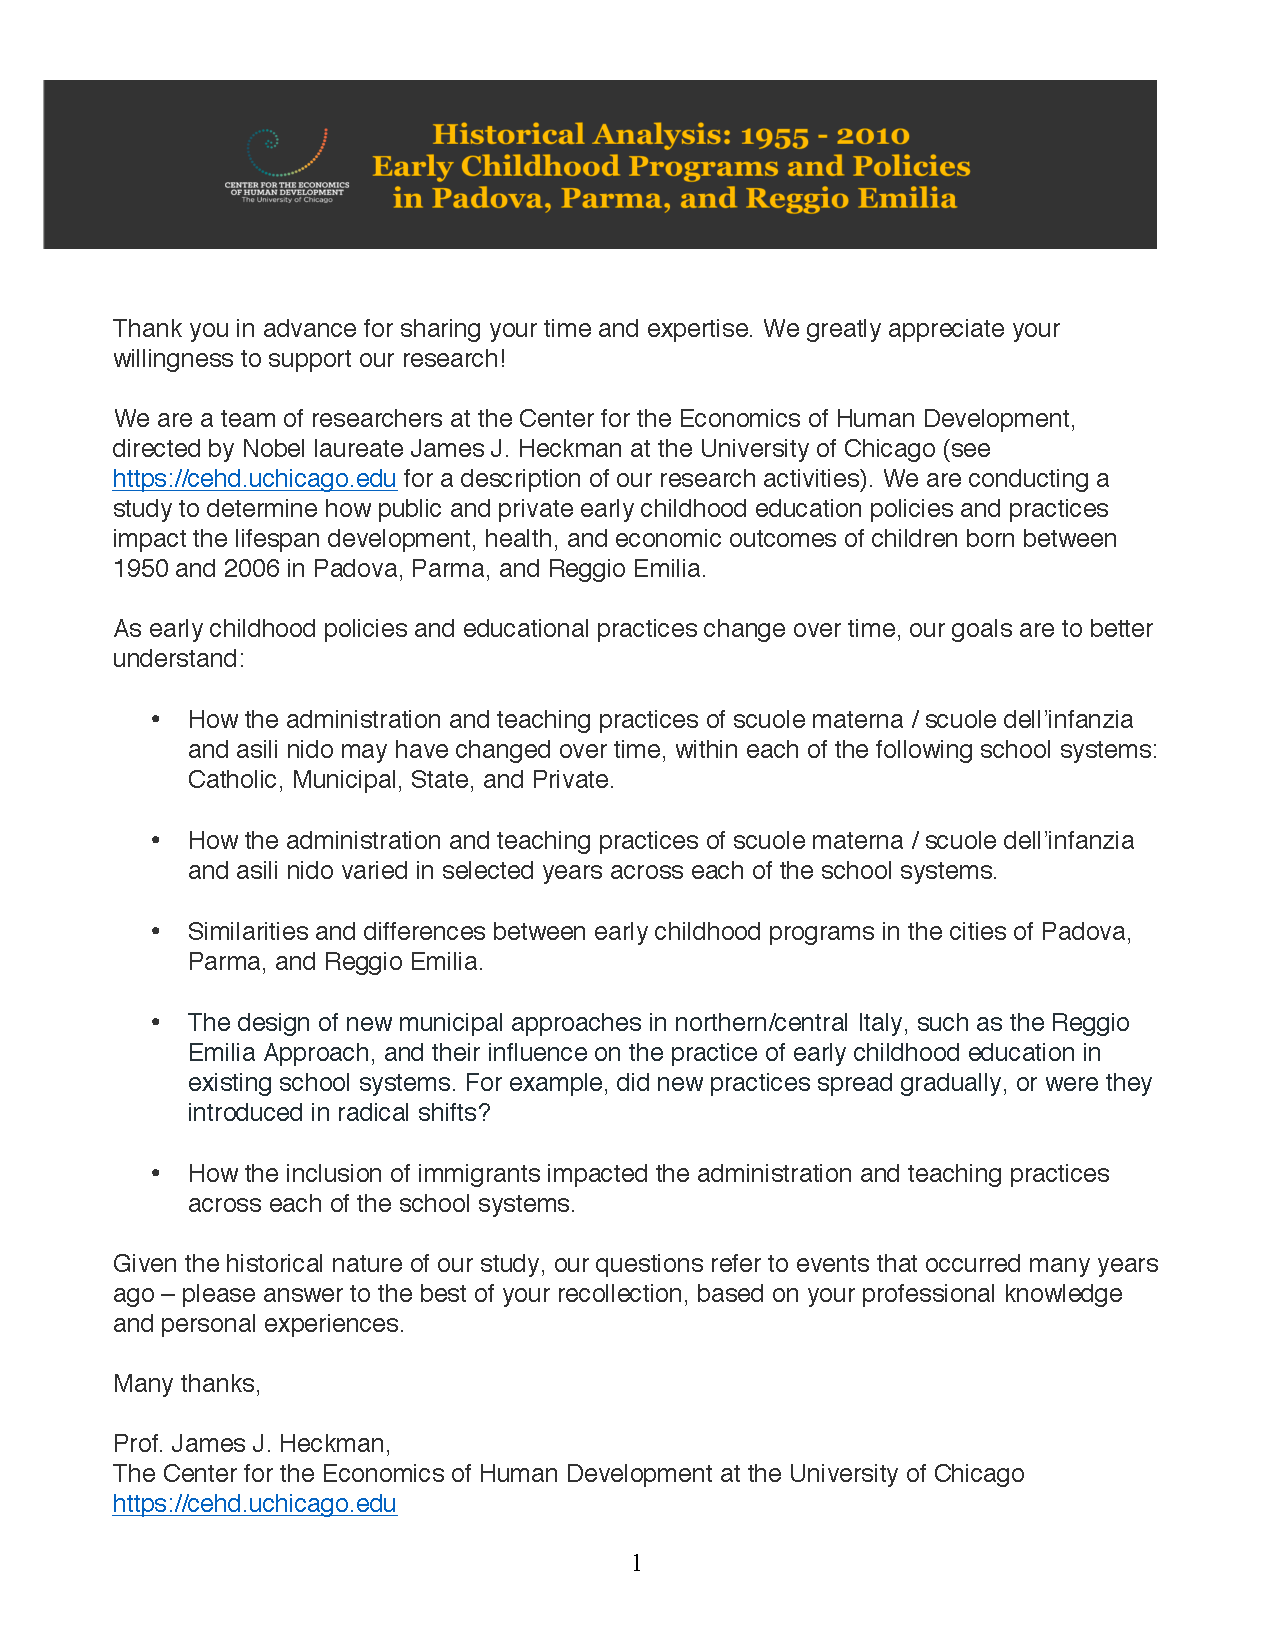
\includepdf[pages=-]{section/CEHD-ECE-Italy_SurveyQuestionnaire-ENGLISH_2016-10-24_sk}

